\chapter{Experimental Results}
\label{chp:results}
BitDF was implemented in C++, using g++ 4.8.4 and the C++11 features. Our experiments were performed in Intel Xeon Quad
Core boxes running Ubuntu Server 14.04. We used four datasets (real and synthetic) in our experiments, with some of them
having more than 50M entries and 2K unique $O_{id}$.

We compare BitDF performance and number of disks generated against an implementation of BFE, using the same datasets
and parameter values. The metrics used for each dataset were (a) CPU time and (b) Number of disks. In (a), for each
flock parameter ($\mu$, $\delta$ and $\epsilon$) we fixed it in a specific value and varied the others, in order to see
how the algorithm behaves. For (b), we analyzed the cumulative number of disks generated over time.

Before showing the results, there are some analysis outcomes that will hold for any dataset analyzed here:

\subsubsection{$\delta$ variation}
\label{sssec:lvariation}
The longer flocks patterns we try to find (long $\delta$), the more disks will stay cached being analyzed and trying to
be merged with new disks from following time slots. This can have a big impact in running time.

\subsubsection{$\epsilon$ variation}
\label{sssec:gvariation}
When the disk radius ($\epsilon$) gets bigger, the more disks will be generated since will be easier to find points that
are "together". And again, the more disks, the more time spent in processing.

\subsubsection{$\mu$ variation}
\label{sssec:nvariation}
By increasing $\mu$, it gets more and more difficult to find disks that are flock candidates ($|D| \ge \mu$), so less
disks are generated. This scenario is where BitDF will achieve less improvements.

\section{Trucks Dataset}
\label{subsec:trucks}
The authors of BFE, modified the dataset in \citep{trucksdataset}. In their modification, every time interval is of
one second, the GPS coordinates were mapped to a $\mathbb{R}^2$ coordinate system (ranging from 0 to 1000) and most of
the points are present in each time interval. The modified dataset resulted in 112203 entries and 276 unique $O_{id}$
(instead of 50 in the original dataset).

\begin{figure*}
    \centering
    \begin{subfigure}[t]{0.25\textwidth}
        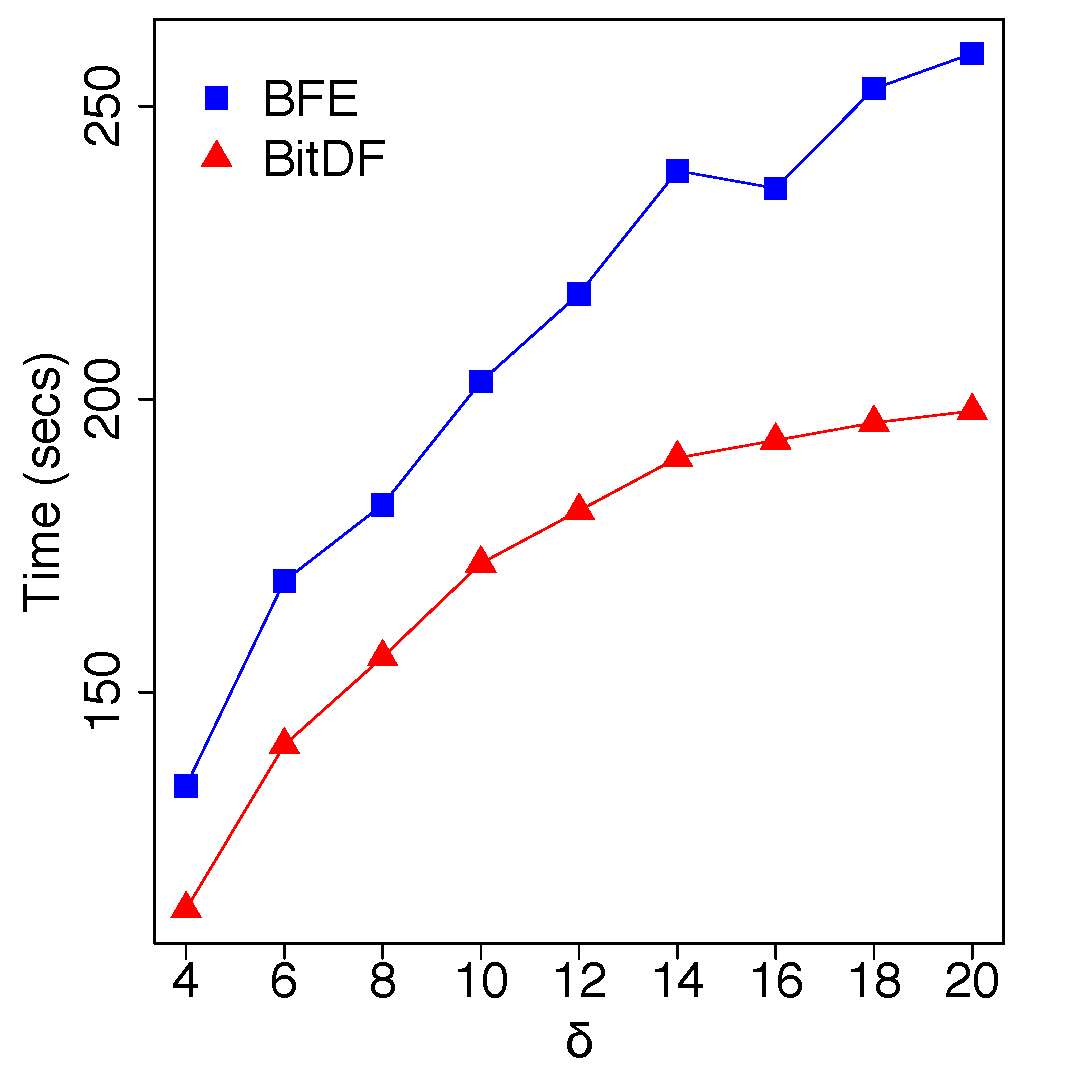
\includegraphics[width=\textwidth]{images/Trucks_n_4_g_1_5_varying_l.eps}
        \caption{$\mu = 4$, $\epsilon = 1.5$ and $\delta$ varying}
        \label{fig:trucks_vary_l}
    \end{subfigure}
    \begin{subfigure}[t]{0.25\textwidth}
        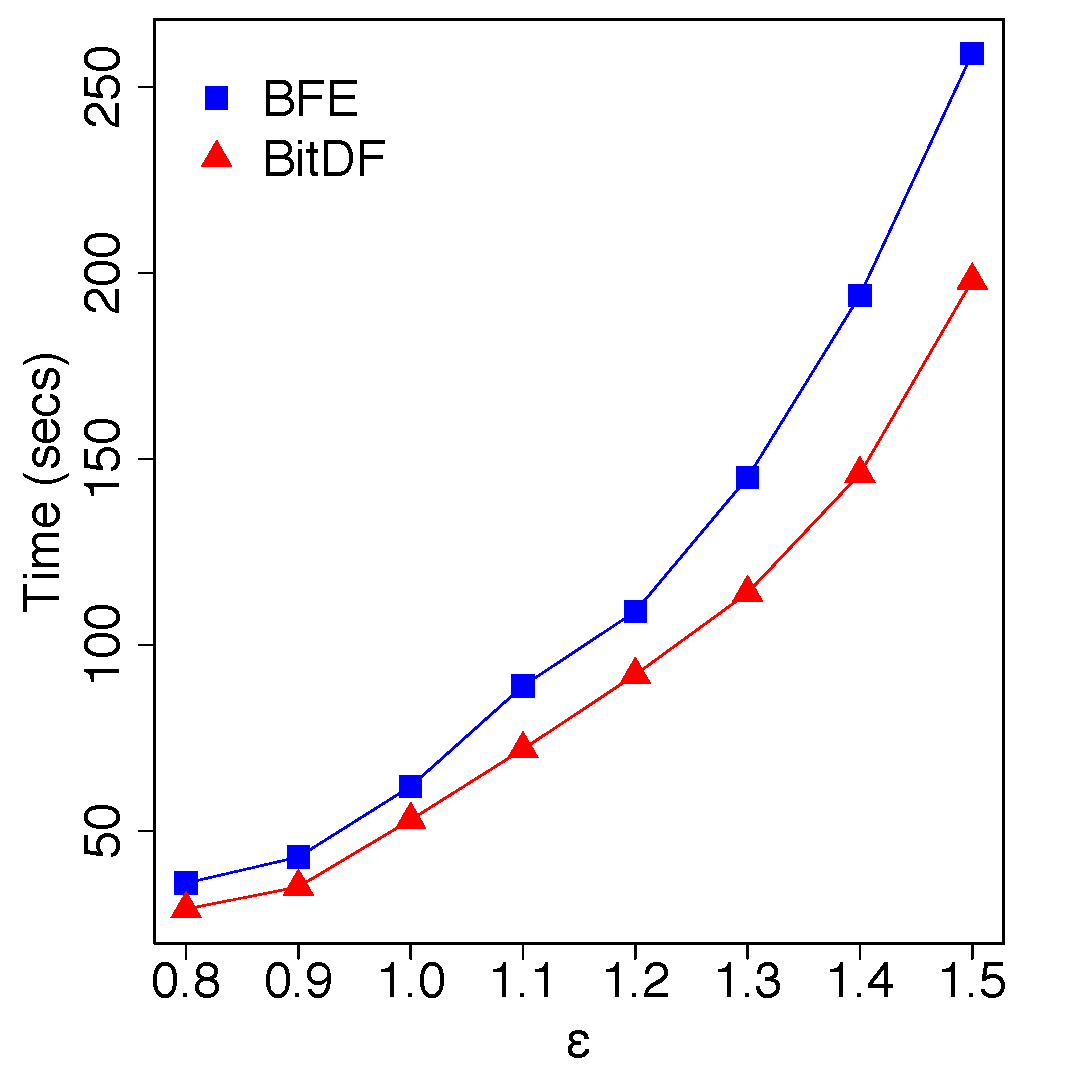
\includegraphics[width=\textwidth]{images/Trucks_n_4_l_20_varying_g.eps}
        \caption{$\mu = 4$, $\delta = 20$ and $\epsilon$ varying}
        \label{fig:trucks_vary_g}
    \end{subfigure}
    \begin{subfigure}[t]{0.25\textwidth}
        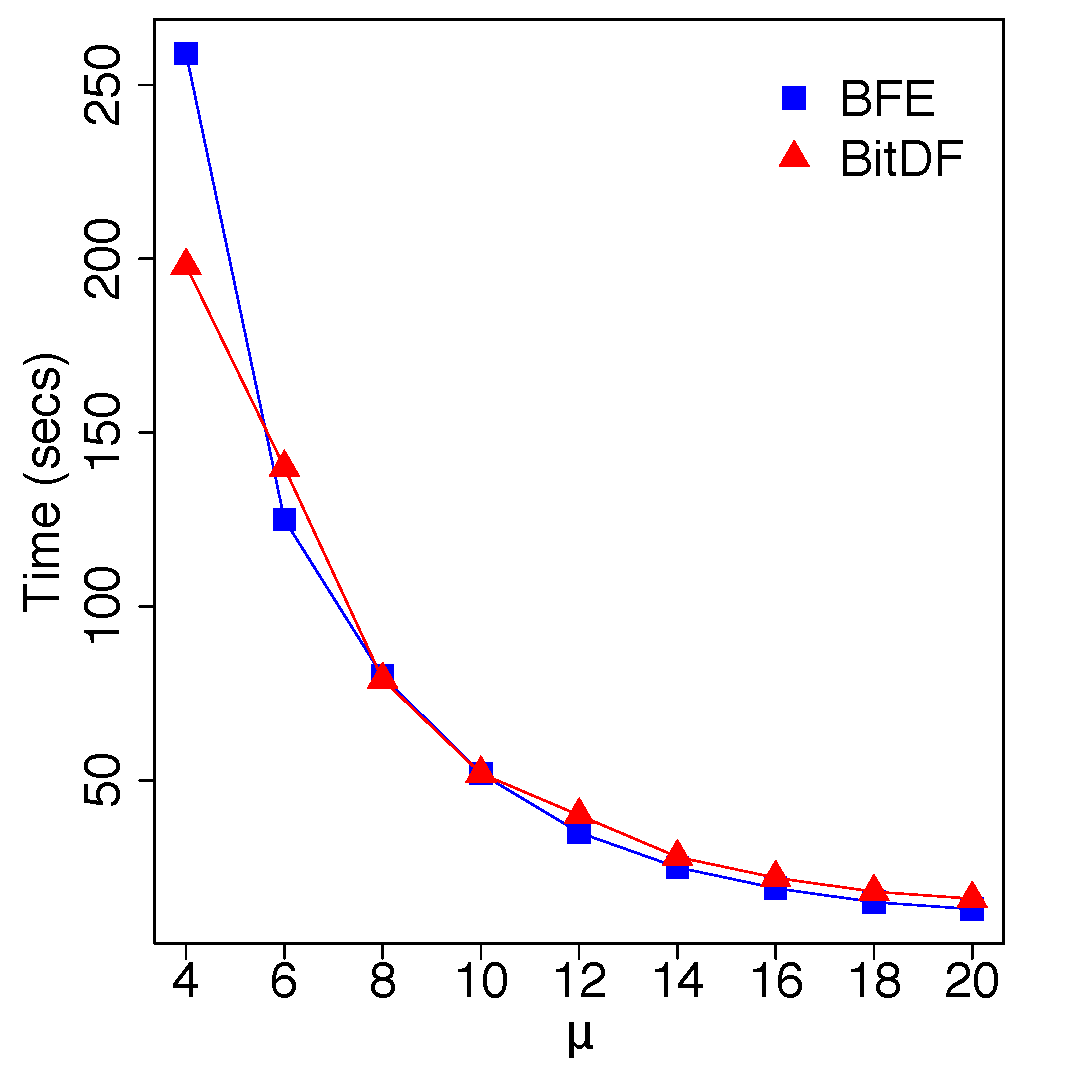
\includegraphics[width=\textwidth]{images/Trucks_l_20_g_1_5_varying_n.eps}
        \caption{$\delta = 20$, $\epsilon = 1.5$ and $\mu$ varying}
        \label{fig:trucks_vary_n}
    \end{subfigure}
    \begin{subfigure}[t]{0.25\textwidth}
        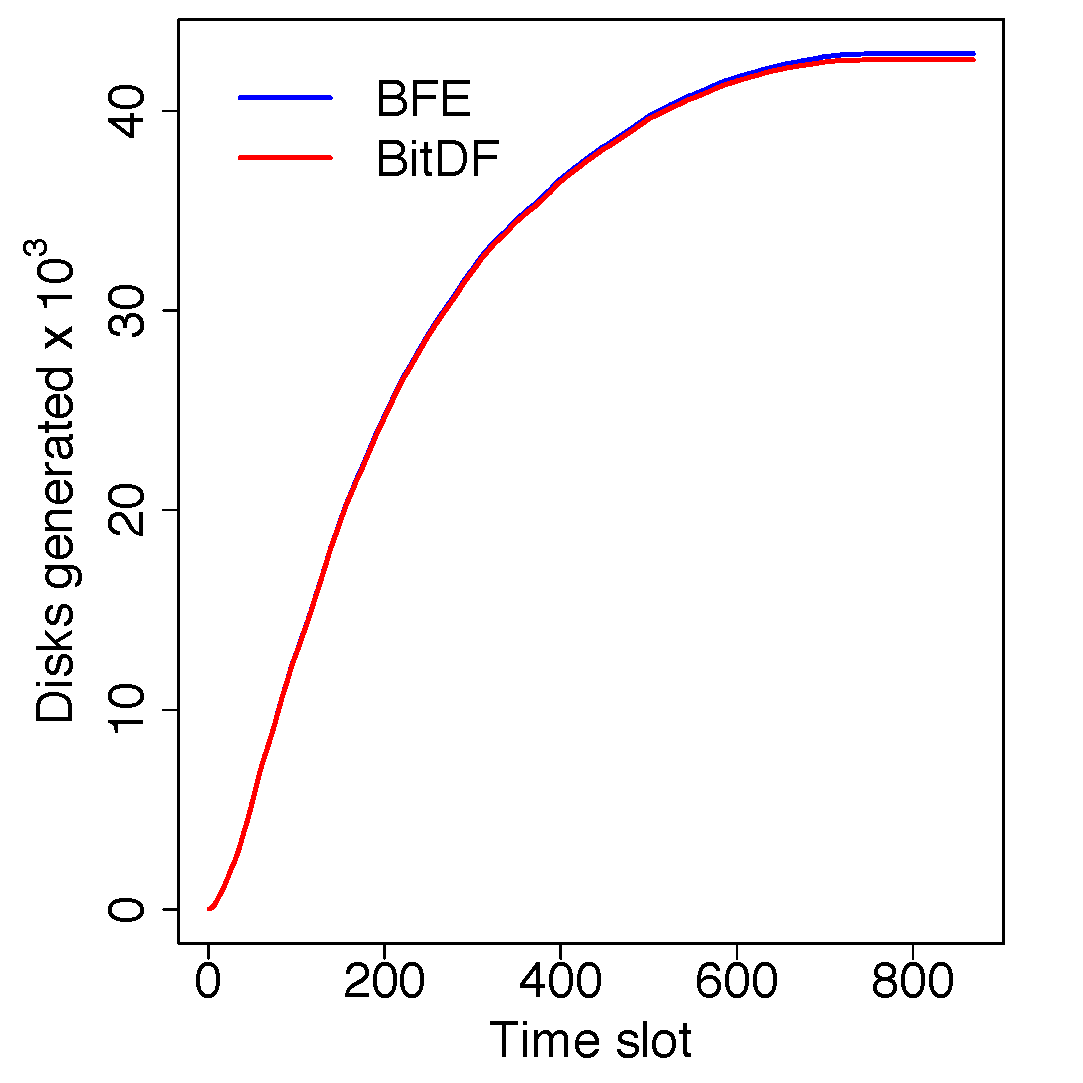
\includegraphics[width=\textwidth]{images/Trucks_d.eps}
        \caption{Cumulative disks by time}
        \label{fig:trucks_disks}
    \end{subfigure}
    \caption{Results for Trucks dataset}
    \label{fig:trucks_results}
\end{figure*}

By looking at Fig. \ref{fig:trucks_results}, we can see that we have some gains in execution time. However, they are not
too significant due to the fact that the number of disks generated by each time slot does not differ too much between
each BFE and BitDF (\ref{fig:trucks_disks}). This happens because almost all points appear in each time slot, then
buffering and mapping the $O_{id}$ presence in time does not make a big impact. We can see some improvements by looking
at Fig. \ref{fig:trucks_vary_l} and Fig. \ref{fig:trucks_vary_g}, which are backed up by the explanations given
at~\ref{sssec:lvariation} and~\ref{sssec:gvariation}. A different behavior is observed in Fig. \ref{fig:trucks_vary_n},
in which BitDF starts better but ends up almost tied with BFE, which can be explained by~\ref{sssec:nvariation}, but is
also very influenced by dataset modifications.

\section{BerlinMOD Dataset}
\label{subsec:berlinmod}
BerlinMOD consists in a traffic generation model \citep{berlinmodpaper} and some synthetic datasets are available in
\citep{berlinmod}. The dataset being analyzed here consists of 56,127,943 entries and 2000 unique $O_{id}$.

As we can see by the results presented in Fig. \ref{fig:berlinmod_results}, BitDF was able to achieve great performance
gains over BFE, in some cases being 57\% faster (Fig. \ref{fig:berlinmod_vary_l}). In \ref{fig:berlinmod_disks} it is
shown that BitDF reduces the cumulative number of disks created over time in 94\%, by only creating disks that can
indeed form flock patterns, which justifies the great improvements that BitDF was able to get in this dataset.
Differently from the results presented in~\ref{subsec:trucks}, even with a growing $\mu$, BitDF was able to get great
improvements over BFE, ranging from 20\% to 48\%.

\begin{figure*}
    \centering
    \begin{subfigure}[t]{0.25\textwidth}
        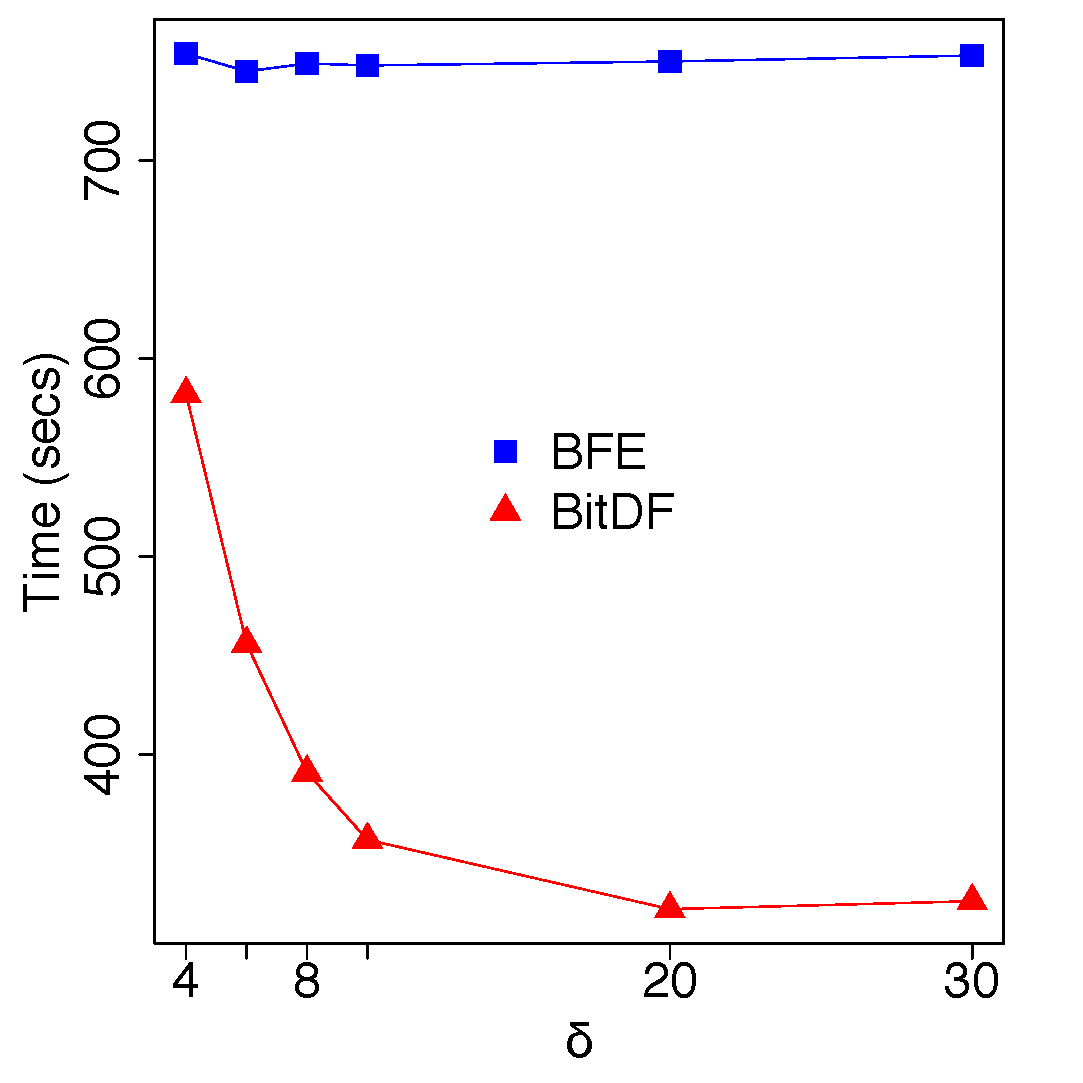
\includegraphics[width=\textwidth]{images/BerlinMOD_n_4_g_100_varying_l.eps}
        \caption{$\mu = 4$, $\epsilon = 100$ and $\delta$ varying}
        \label{fig:berlinmod_vary_l}
    \end{subfigure}
    \begin{subfigure}[t]{0.25\textwidth}
        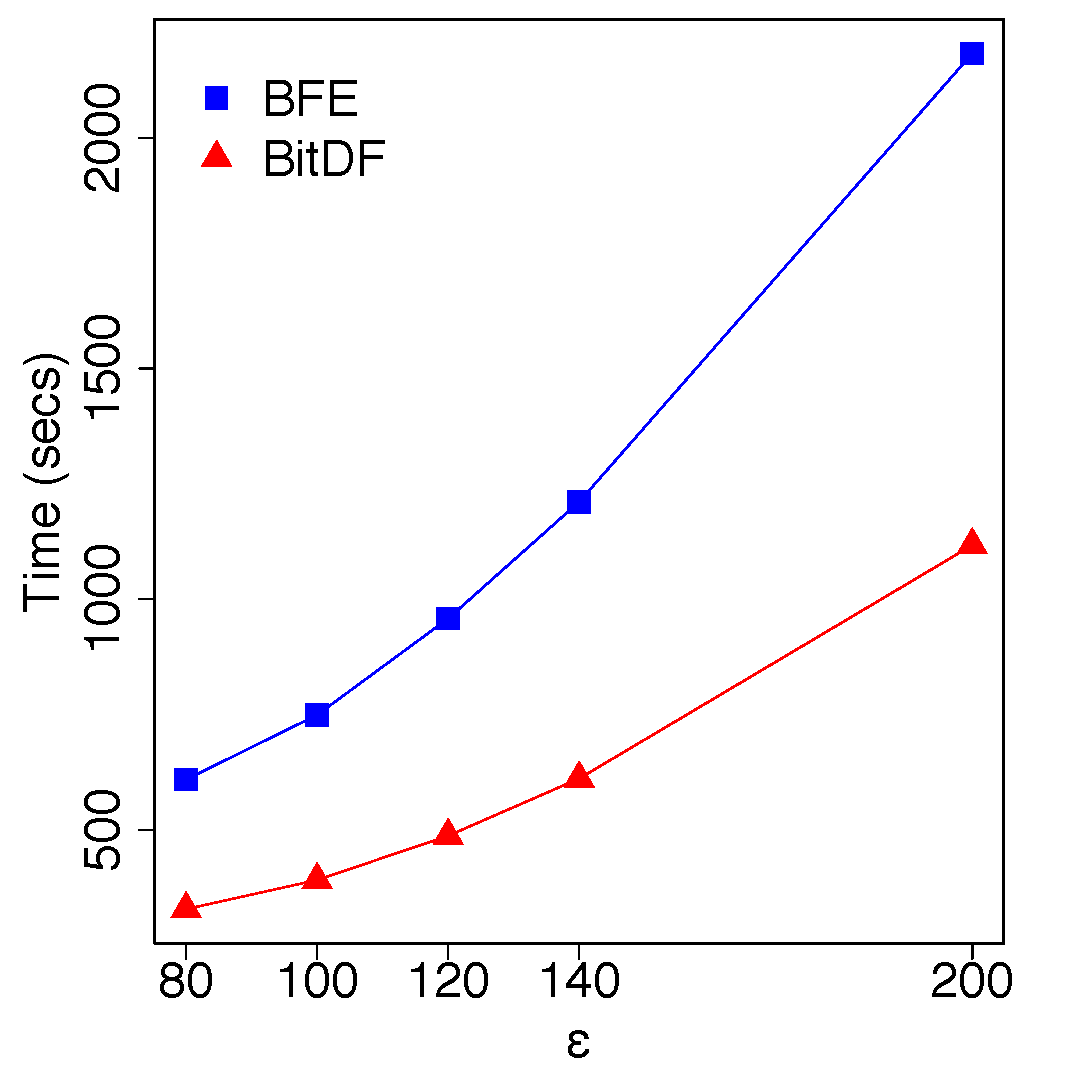
\includegraphics[width=\textwidth]{images/BerlinMOD_n_4_l_8_varying_g.eps}
        \caption{$\mu = 4$, $\delta = 8$ and $\epsilon$ varying}
        \label{fig:berlinmod_vary_g}
    \end{subfigure}
    \begin{subfigure}[t]{0.25\textwidth}
        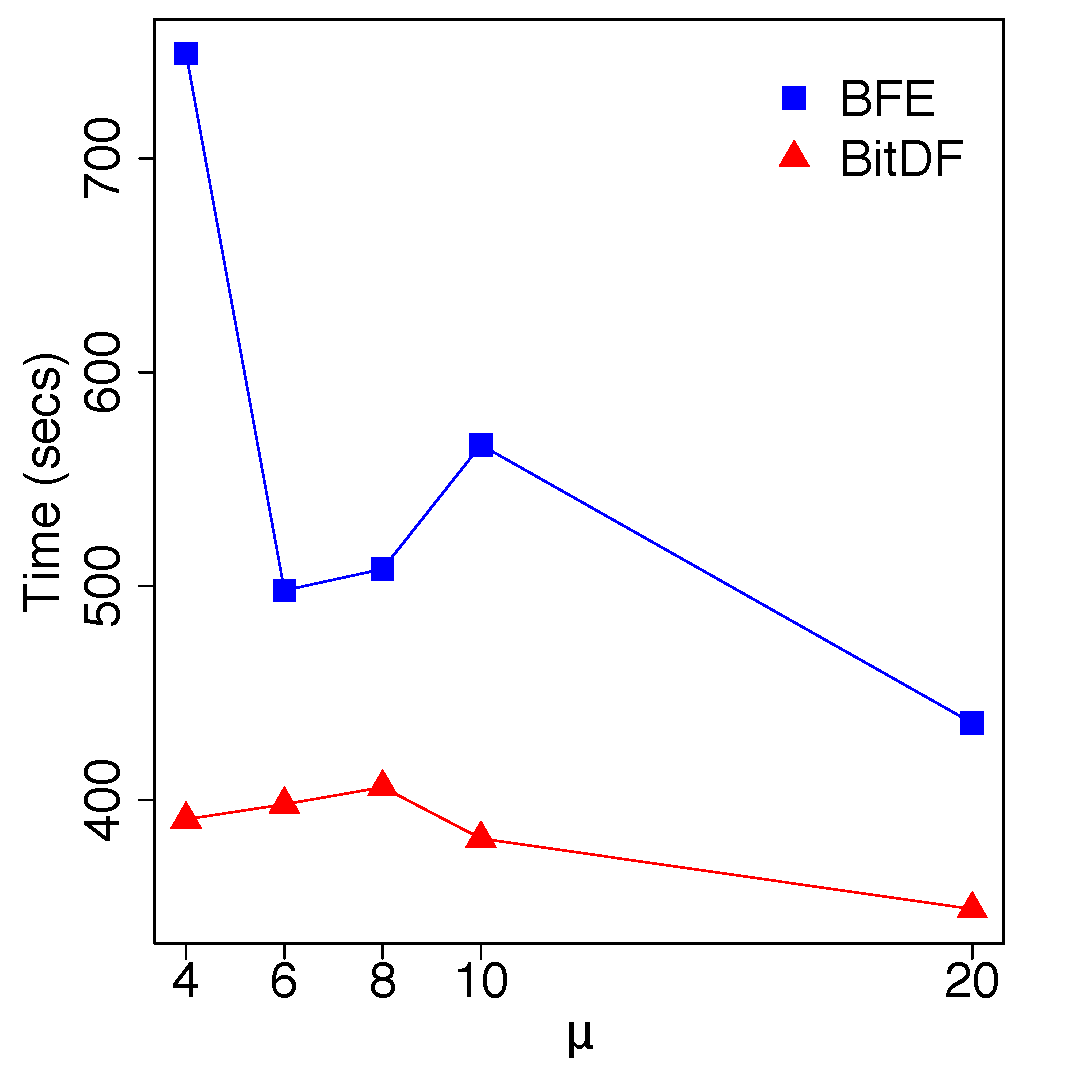
\includegraphics[width=\textwidth]{images/BerlinMOD_l_8_g_100_varying_n.eps}
        \caption{$\delta = 8$, $\epsilon = 100$ and $\mu$ varying}
        \label{fig:berlinmod_vary_n}
    \end{subfigure}
    \begin{subfigure}[t]{0.25\textwidth}
        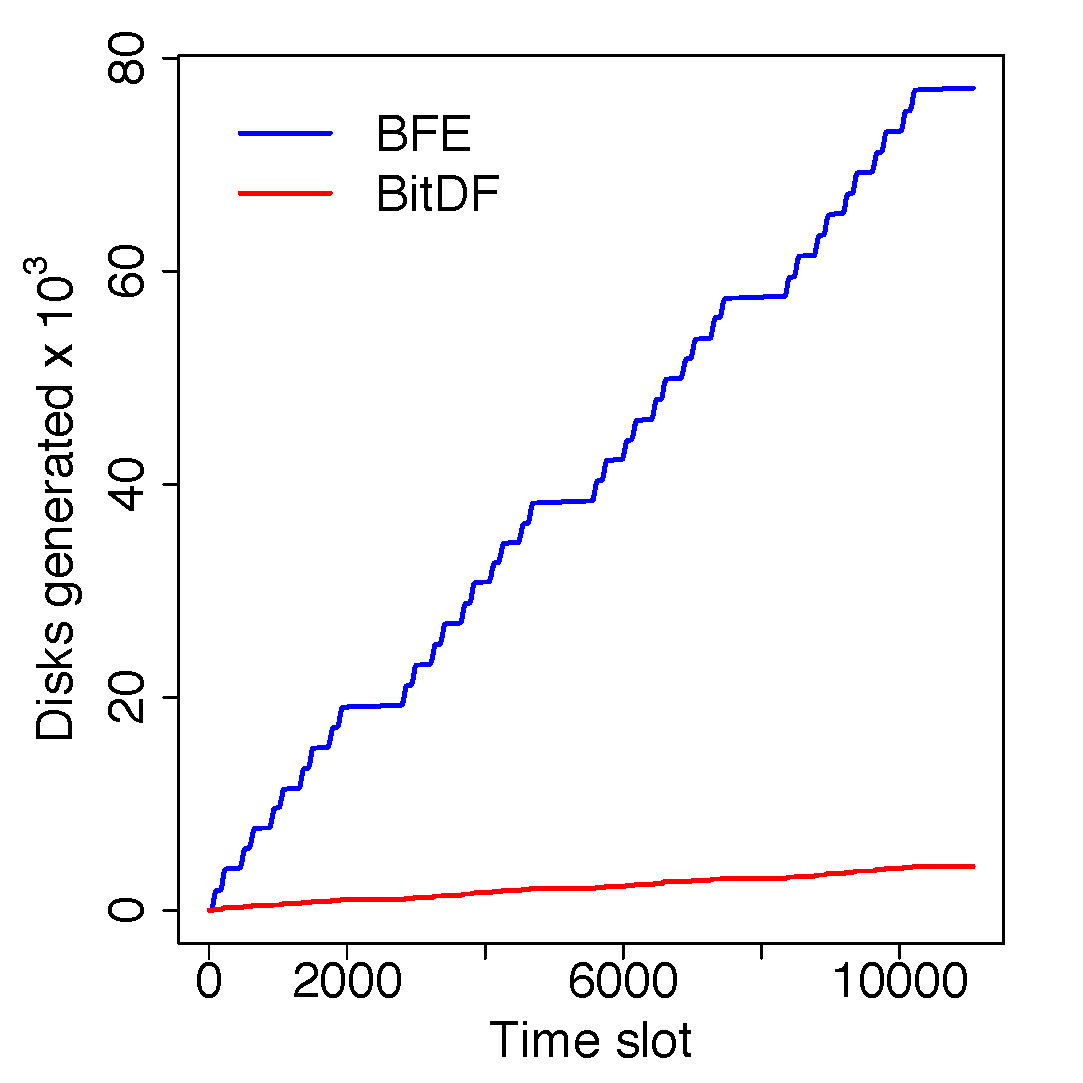
\includegraphics[width=\textwidth]{images/BerlinMOD_d.eps}
        \caption{Cumulative disks by time}
        \label{fig:berlinmod_disks}
    \end{subfigure}
    \caption{Results for BerlinMOD dataset}
    \label{fig:berlinmod_results}
\end{figure*}

\section{TDrive Dataset}
\label{subsec:tdrive}
This is a real dataset, having spatio-temporal data describing trajectories of taxis in Beijing, China, available in
\citep{tdrive}. It has 17,762,489 entries with 10336 $O_{id}$.

As reported in Fig. \ref{fig:tdrive_results}, BitDF was able to dramatically reduce the execution time when varying the
$\delta$ parameter, reaching almost 90\% of improvement. Likewise, BitDF reduced the execution time up to 74\% when
varying $\epsilon$. However, despite seeing some similar behavior with the other analyzed datasets when varying $\mu$,
BitDF was able to improve the execution time by 74\% in some cases. It is also worth noting that the results achieved
are a reflex of the huge decrease of disks, as depicted in Fig. \ref{fig:tdrive_disks}, in which we can see an reduction
of 96\%.

\begin{figure*}
    \centering
    \begin{subfigure}[t]{0.25\textwidth}
        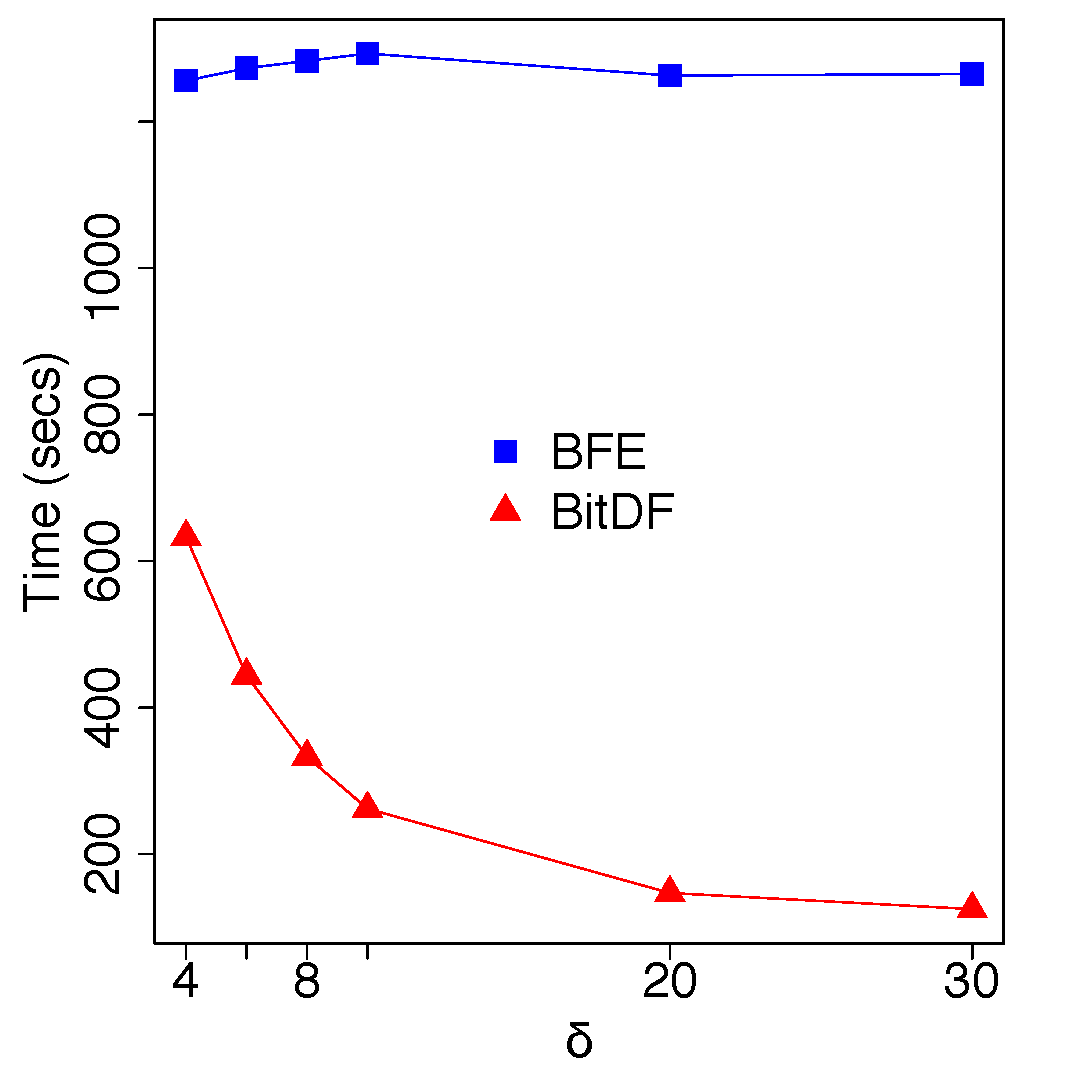
\includegraphics[width=\textwidth]{images/TDrive_n_4_g_100_varying_l.eps}
        \caption{$\mu = 4$, $\epsilon = 100$ and $\delta$ varying}
        \label{fig:tdrive_vary_l}
    \end{subfigure}
    \begin{subfigure}[t]{0.25\textwidth}
        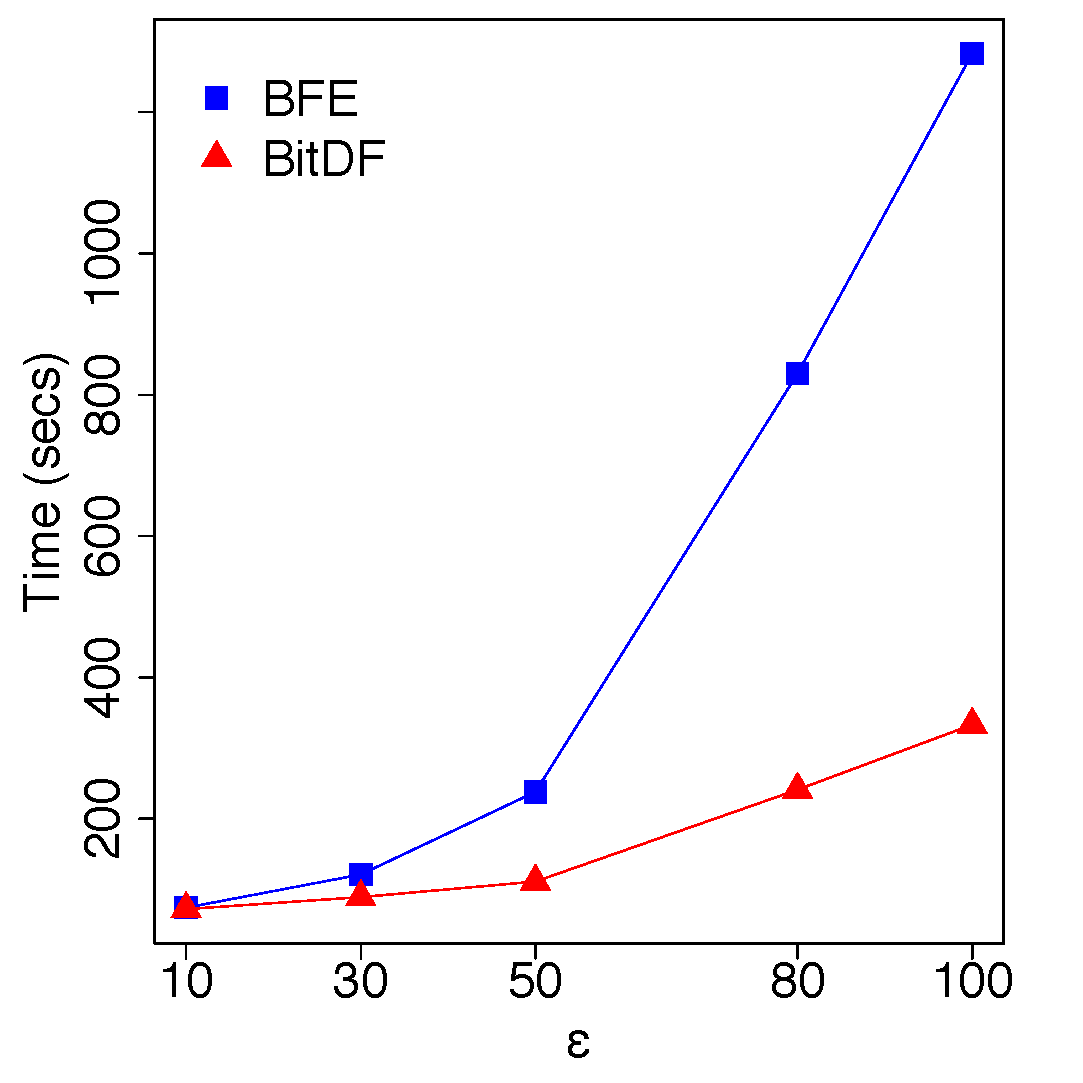
\includegraphics[width=\textwidth]{images/TDrive_n_4_l_8_varying_g.eps}
        \caption{$\mu = 4$, $\delta = 8$ and $\epsilon$ varying}
        \label{fig:tdrive_vary_g}
    \end{subfigure}
    \begin{subfigure}[t]{0.25\textwidth}
        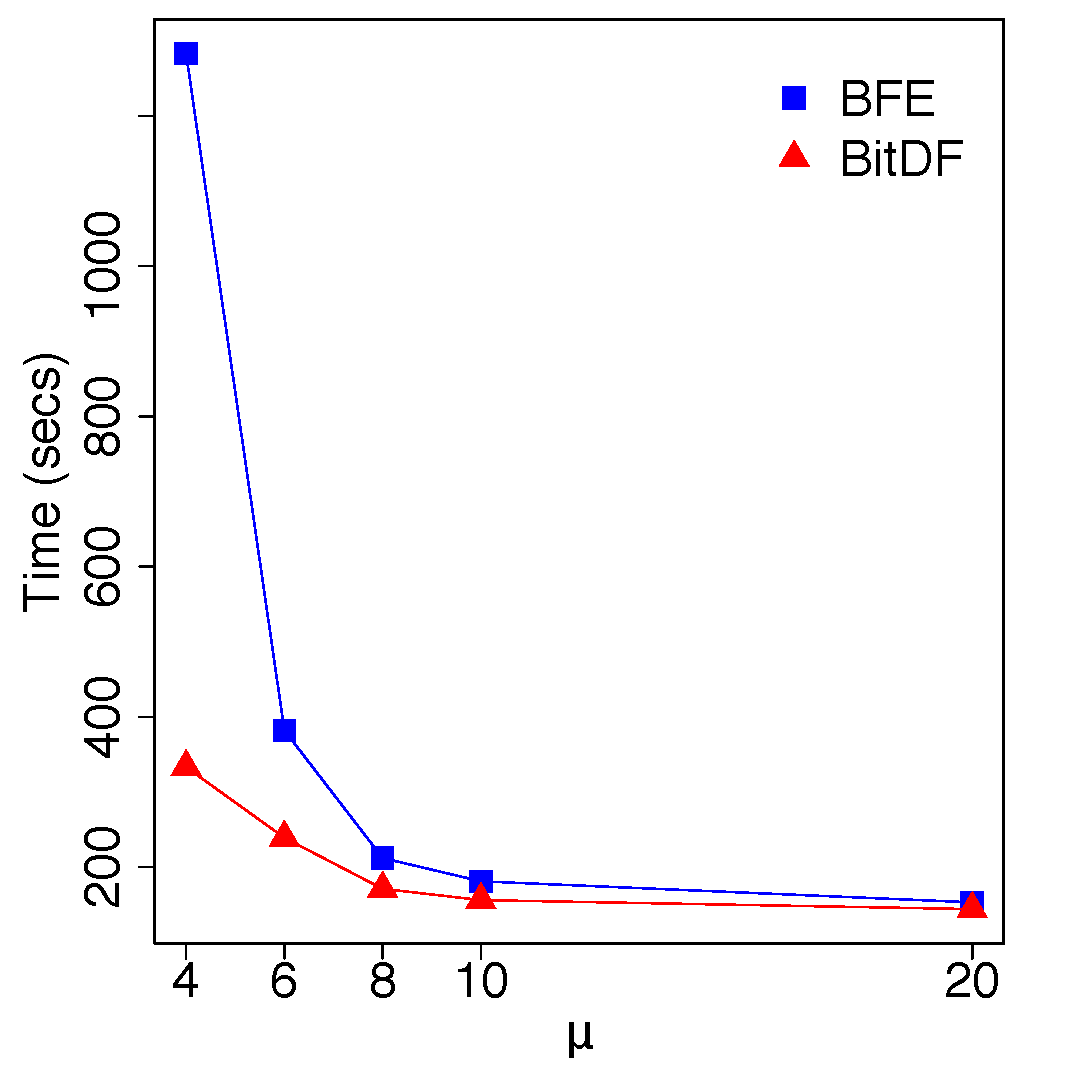
\includegraphics[width=\textwidth]{images/TDrive_l_8_g_100_varying_n.eps}
        \caption{$\delta = 8$, $\epsilon = 100$ and $\mu$ varying}
        \label{fig:tdrive_vary_n}
    \end{subfigure}
    \begin{subfigure}[t]{0.25\textwidth}
        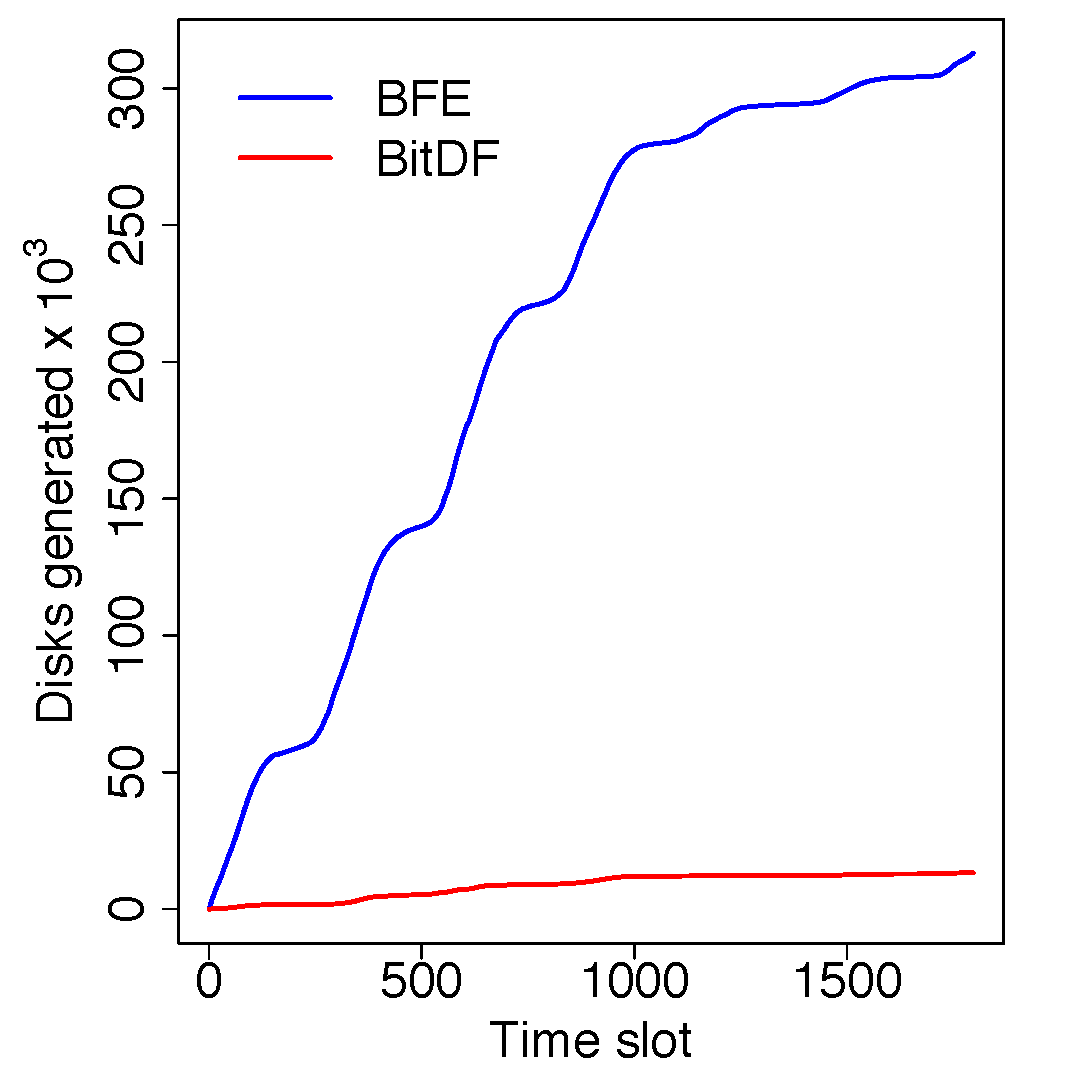
\includegraphics[width=\textwidth]{images/TDrive_d.eps}
        \caption{Cumulative disks by time}
        \label{fig:tdrive_disks}
    \end{subfigure}
    \caption{Results for TDrive dataset}
    \label{fig:tdrive_results}
\end{figure*}

\section{Brinkkhoff Dataset}
\label{subsec:brinkhoff}
Likewise BerlinMOD, Brinkhoff is also a city traffic generation model \citep{brinkhoffpaper}. We generated a
synthetic dataset using the Minnesota Web-based Traffic Generator \citep{mntg}, having 2000 as the "Starting
Vehicles" and 100 as the "Simulation Time" parameters. The result dataset has 314,523 entries and 7000 unique $O_{id}$.

Fig. \ref{fig:brinkhoff_results} shows how good BitDF performed against this dataset, having improvements up to 99\% for
both $\delta$ and $\epsilon$ parameters variation. Even with the variation of $\mu$, BitDF was able to show huge
improvement, with results ranging from 98\% to 85\% of CPU time reduction. Additionally, we can see in Fig.
\ref{fig:brinkhoff_disks} that we were able to reduce the number of disks by 95\%, what is a huge improvement and is
reflecting directly in the running time of BitDF.

\begin{figure*}
    \centering
    \begin{subfigure}[t]{0.25\textwidth}
        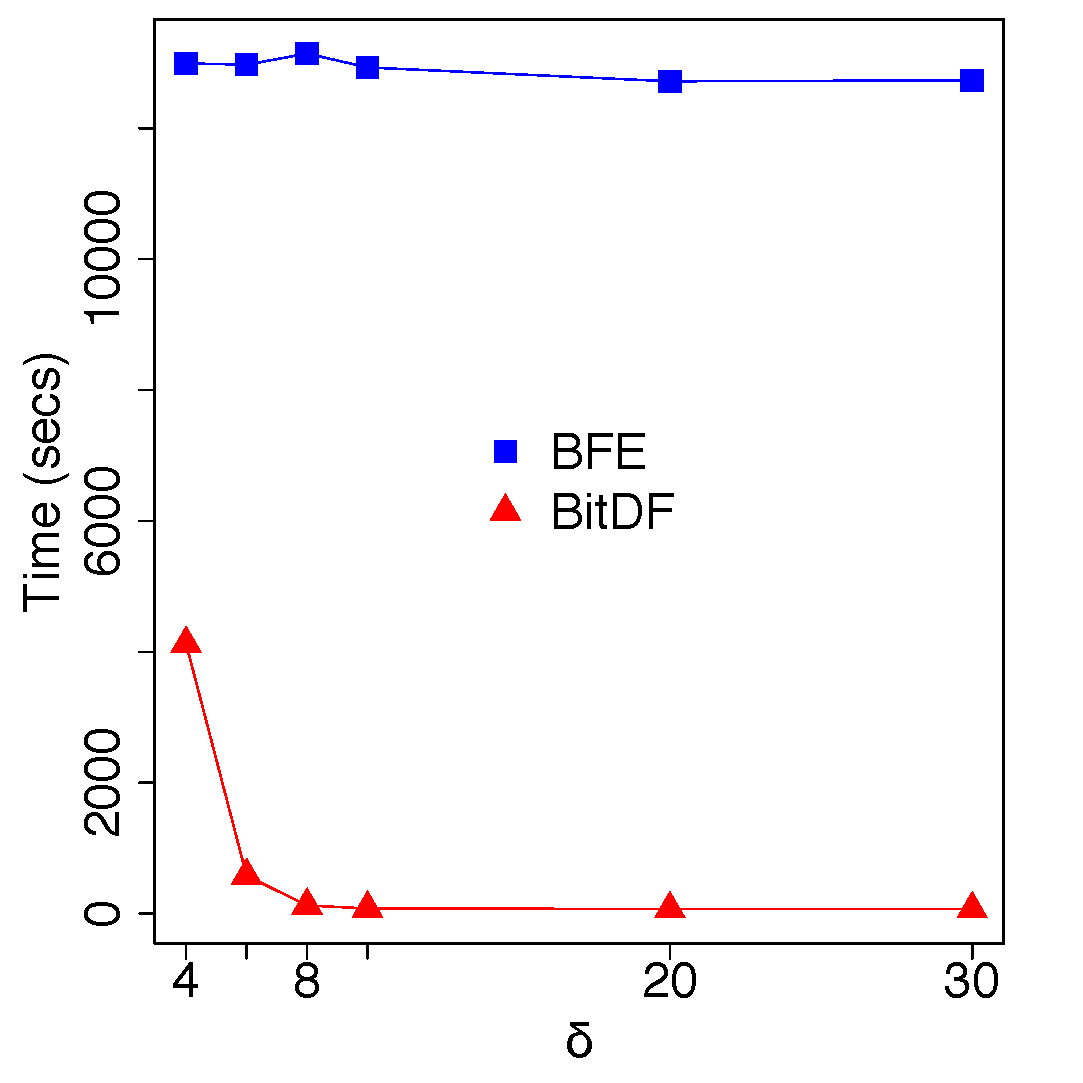
\includegraphics[width=\textwidth]{images/Brinkhoff_n_4_g_200_varying_l.eps}
        \caption{$\mu = 4$, $\epsilon = 100$ and $\delta$ varying}
        \label{fig:brinkhoff_vary_l}
    \end{subfigure}
    \begin{subfigure}[t]{0.25\textwidth}
        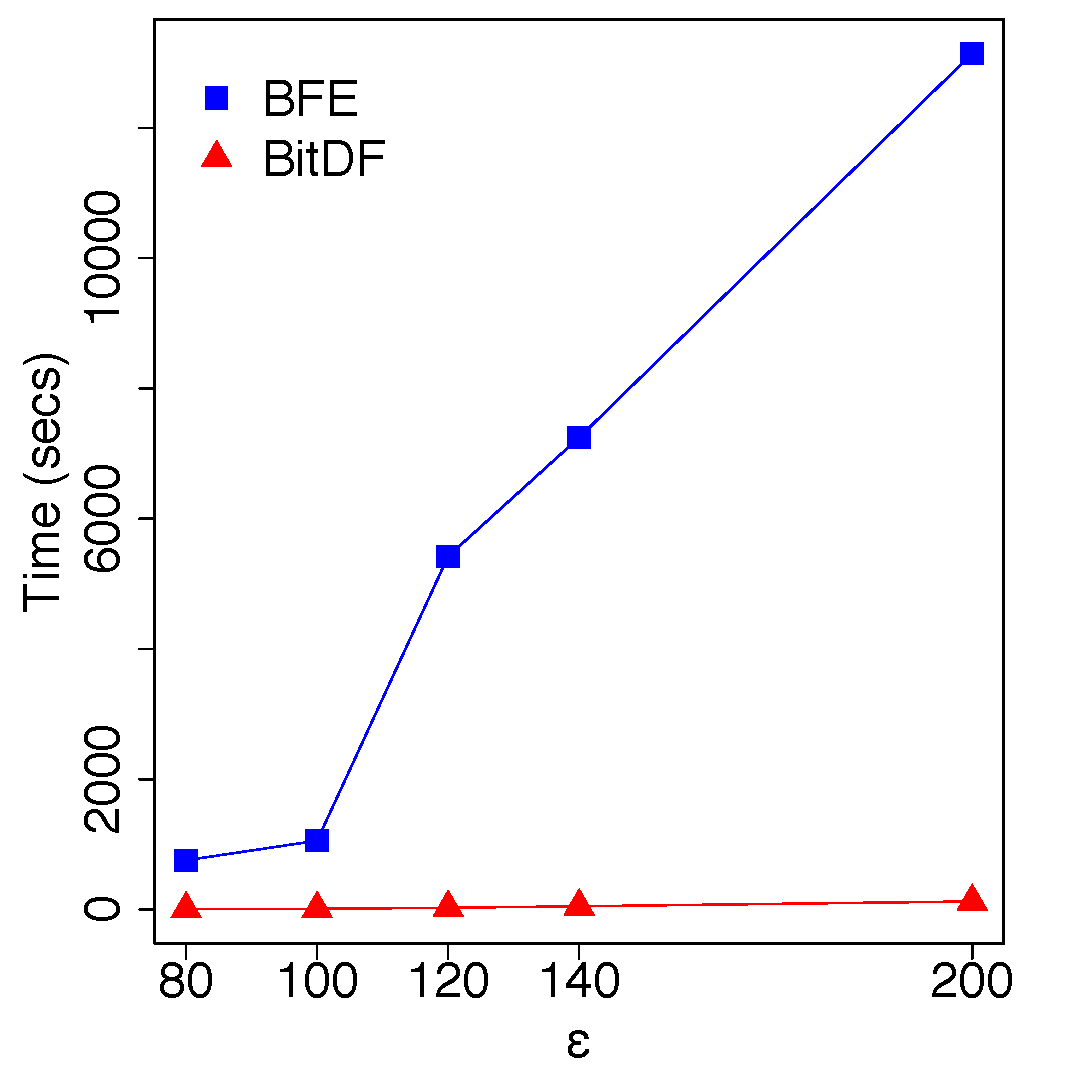
\includegraphics[width=\textwidth]{images/Brinkhoff_n_4_l_8_varying_g.eps}
        \caption{$\mu = 4$, $\delta = 8$ and $\epsilon$ varying}
        \label{fig:brinkhoff_vary_g}
    \end{subfigure}
    \begin{subfigure}[t]{0.25\textwidth}
        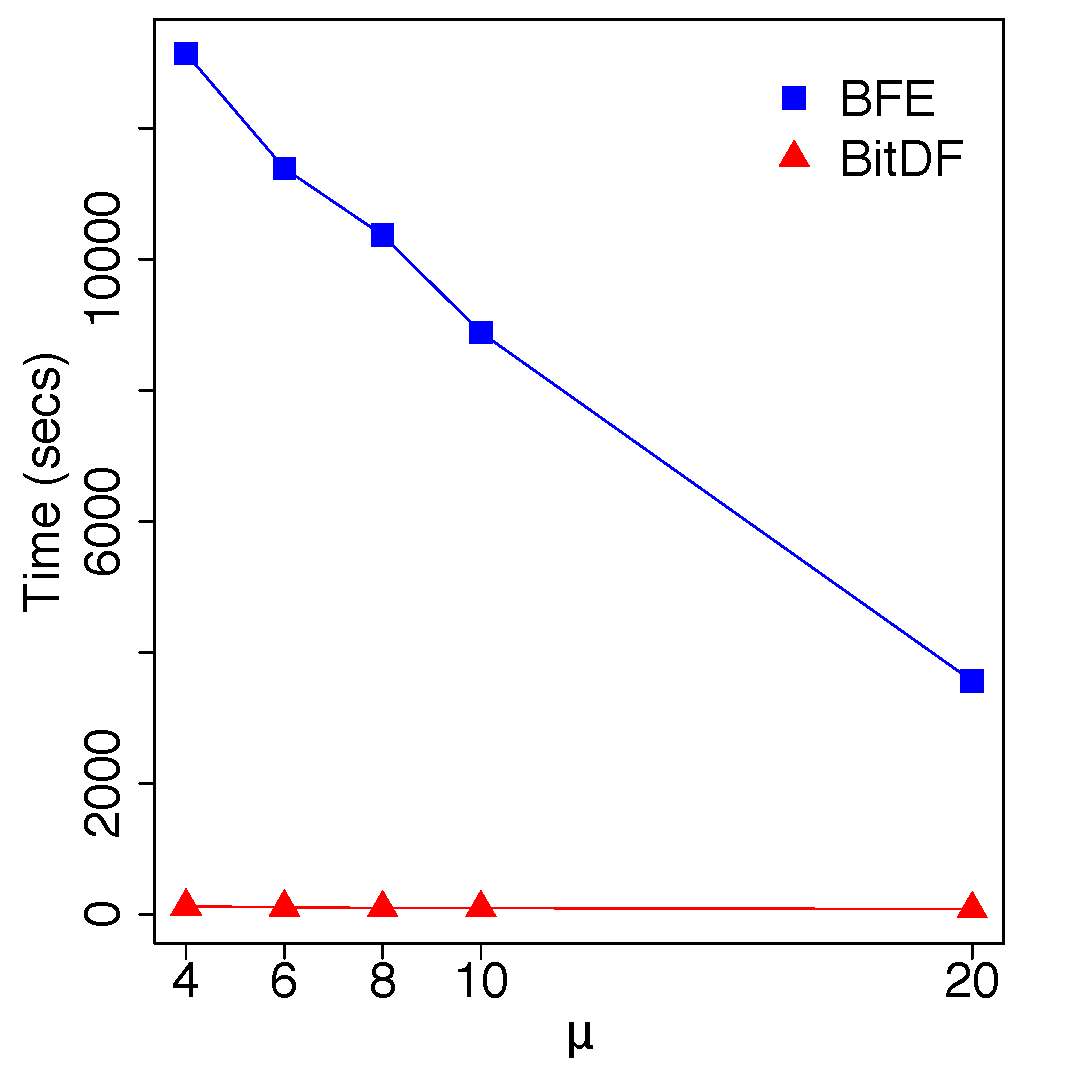
\includegraphics[width=\textwidth]{images/Brinkhoff_l_8_g_200_varying_n.eps}
        \caption{$\delta = 8$, $\epsilon = 100$ and $\mu$ varying}
        \label{fig:brinkhoff_vary_n}
    \end{subfigure}
    \begin{subfigure}[t]{0.25\textwidth}
        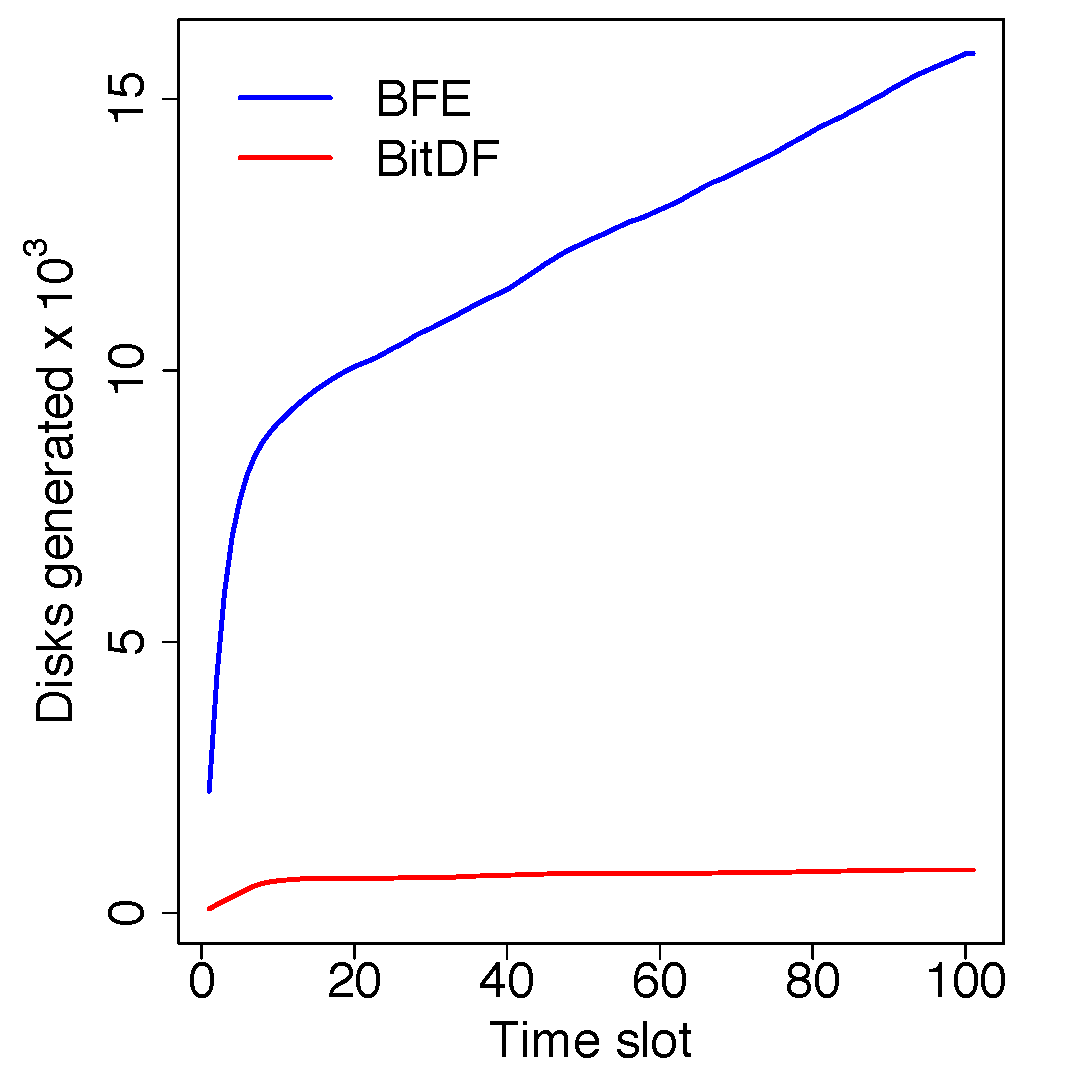
\includegraphics[width=\textwidth]{images/Brinkhoff_d.eps}
        \caption{Cumulative disks by time}
        \label{fig:brinkhoff_disks}
    \end{subfigure}
    \caption{Results for Brinkhoff dataset}
    \label{fig:brinkhoff_results}
\end{figure*}
